\documentclass[a4paper, 12pt]{article}
%\usepackage[polish]{babel}
%\usepackage[cp1250]{inputenc}
\usepackage[latin2]{inputenc}
%\usepackage{polski}
\usepackage[T1]{fontenc}
\usepackage{graphicx}


\pagestyle{headings}
\textwidth      15.5cm
\oddsidemargin    .1cm
\evensidemargin   .1cm



\begin{document}

\thispagestyle{empty}

\begin{minipage}{5cm}
%
\includegraphics[scale=0.3]{logo.eps}
\end{minipage}
\begin{minipage}{10cm}
\begin{center}
{Salomon\\
System przetwarzania wiedzy\\}
\end{center}
\end{minipage}

\vspace*{0.5cm}

\hrulefill

\vspace*{1cm}


\begin{flushleft}

\section{Drzewa decyzyjne w teorii decyzji}

W teorii decyzji drzewo decyzyjne jest drzewem decyzji i ich mozliwych konsekwencji (stan�w natury). Zadaniem drzew decyzyjnych mo�e by� zar�wno stworzenie planu, jak i rozwiazanie problemu decyzyjnego.

Metoda drzew decyzyjnych jest szczeg�lnie przydatna w problemach decyzyjnych z licznymi, rozga�eziajacymi sie wariantami oraz w przypadku podejmowania decyzji w warunkach ryzyka.

\section{Drzewa decyzyjne w uczeniu maszynowym}

Drzewa decyzyjne w uczeniu maszynowym s�uza do wyodrebniania wiedzy z zestawu przyk�ad�w (patrz eksploracja danych). Zak�adamy, ze posiadamy zestaw przyk�ad�w: obiekt�w opisanych przy pomocy atrybut�w, kt�rym przyporzadkowujemy jakas decyzje (patrz tabela decyzyjna).

Przyk�ad: Chcemy zautomatyzowa� proces przyjmowania kandydat�w na praktyki w duzej firmie. Posiadamy setki przyk�ad�w z przesz�osci, chcemy wydoby� z nich regu�y decyzyjne. Atrybuty Wykszta�cenie, Jezyki obce, Doswiadczenie i Og�lne wrazenie sa kodowane skala od 1 do 5.
\linebreak
%do poprawy
\begin{table}[h]
%\multicolumn{7}{c}{	}
Wiek 	P�e� 	Wykszta�cenie 	Jezyki 	Doswiadczenie 	Prezentacja 	Przyjety\linebreak 
25 	m 	2 	4 	1 	4 	nie\linebreak 
22 	k 	4 	3 	4 	2 	nie\linebreak 
21 	m 	4 	5 	5 	4 	tak\linebreak 
29 	m 	1 	3 	2 	3 	nie\linebreak 
\caption{}
\end{table} 
\linebreak
Na podstawie tabeli decyzyjnej tworzymy drzewo, kt�rego wez�ami sa poszczeg�lne atrybuty, ga�eziami wartosci odpowiadajace tym atrybutom, a liscie tworza poszczeg�lne decyzje. Na podstawie przyk�adowych danych wygenerowano nastepujace drzewo:

	\begin{center}
	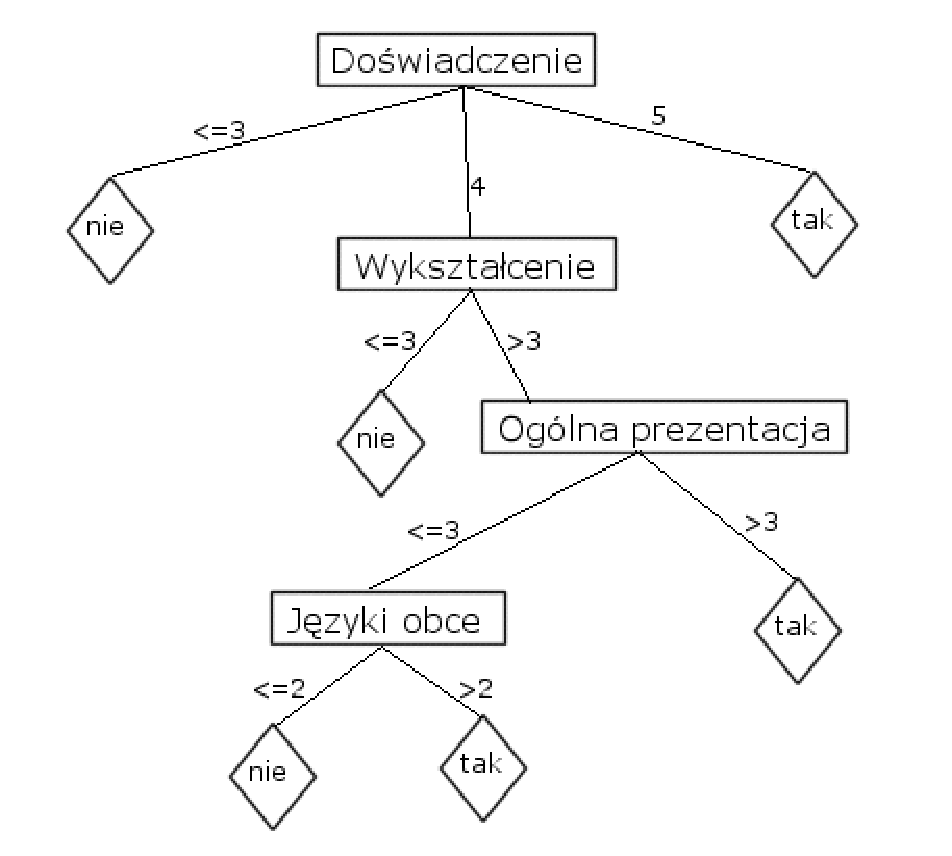
\includegraphics[bb=0 447 441 842]{dd.eps}
% dd.eps: 300dpi, width=3.73cm, height=3.34cm, bb=0 447 441 842
	\end{center}

Drzewo w takiej postaci odzwierciedla w jaki spos�b na podstawie atrybut�w by�y podejmowane decyzje klasyfikujace (dla uproszczenia po�aczono niekt�re ga�ezie). Zaleta tej reprezentacji jest jej czytelnos� dla cz�owieka. W prosty spos�b mozna przekszta�ci� ja do reprezentacji regu�owej.

\section{Algorytm tworzenia drzewa ID3}
\subsection{Wstep}
Algorytm tworzenia drzew decyzyjnych ID3 jest jednym z prostszych algorytmow ale zarazem daje on dosc dobre wyniki. Celem jest oczywiscie stworzenie drzewa, ktore za pomoca wartosci atrybutow przyjmowanych przez elementy podzieli nam dziedzine na klasy rownowaznosci (w domysle podgrupy majace taka sama wartosc jednej ze zmiennych). Oczywiscie w typowym przypadku mozliwosci stworzenia takiego drzewa bedzie wiele. Wiec ustalamy dodatkowy cel, jakim bedzie minimalna wysokosc drzewa, liczona jako najwieksza odleglosc od korzenia do liscia. Algorytm ID3 zawsze (jezeli to mozliwe) stworzy nam drzewo decyzyjne. Natomiast nie zawsze jest to drzewo optymalnej wielkosci. Algorytm ID3 jest algorytmem zach�annym, decyzje o rozbudowie drzewa sa podejmowane na podstawie przyblizonej oceny kazdego z wariantow jakie mozemy przyjac w danym kroku. Raz podjeta decyzja nie jest juz zmieniana - nie jest to algorytm adaptatywny. Przyjrzyjmy sie jego dzialaniu.

\subsection{Informacje wstepne}
Na wejsciu algorytm dostaje zestaw danych, zwanych "test cases". Przy pomocy tych danych bedzie budowane drzewo decyzyjne. Danymi sa rekordy posiadajace wiele atrybutow. Konieczne jest okreslenie ktory z atrybutow jest artybutem wzgledem ktorego bedziemy tworzyc drzewo decyzyjne. W zamieszczonym wczesniej przykladzie jest to fakt przyjecia lub nieprzyjecia kandydata do pracy. Milczacym zalozeniem jest ze pozostale atrybuty maja byc brane pod uwage przy tworzeniu drzewa decyzyjnego. 
Drzewo sklada sie z zestawu wezlow i lisci. Wezly w stworzonym drzewie beda reprezentowac testy wartosci atrybutu a liscie beda podjetymi decyzjami. Odnoszac to do opisanego wczesniej przypadku mozna powiedziec ze np. test wartosci wspolczynnika okreslajacego znajomosc jezykow obcych (podzial na rekordy <=2 i >2) jest wezlem drzewa a decyzja ze kandydat zostal przyjety jest jego lisciem.
Poczatkowo drzewo sklada sie z jednego tylko liscia do ktorego przypiete sa wszystkie "test cases". 

Oznaczmy:
\begin{itemize}
\item nb, liczba instancji w lisciu b
\item nbc, liczba instancji w lisciu b nalezacych do klasy c. nbc <= nb
\item nt, calkowita liczna instancji we wszystkich lisciach
\end{itemize}

Teraz przy pomocy tych oznaczen mozemy zapisac podstawowe wzory prawdopodobiensta:
$P_{b}=\frac{n_{bc}}{n_{b}}$
\begin{itemize}
\item Jezeli wszystkie instancje w grupie sa klasyfikowane pozytywnie, wtedy Pb = 1 (lisc homogeniczny pozytywnie) 
\item Jezeli wszystkie instancje w grupie sa klasyfikowane negatywnie, wtedy Pb = 0 (lisc homogeniczny negatywnie) 
\end{itemize}

Bazujac na tym zapisie prawdopodobienstwa zdefiniujejmy sobie formule entropii - bedzie nam ona potrzebna pozniej, przy tworzeniu drzewa decyzyjnego.

\subsubsection{Entropia}
Entropia jest miara z teorii informacji, charakteryzujaca czystosc i homogenicznosc zbioru atrybutow. 
$Entropia = Sum(c)(-\frac{n_{bc}}{n_{b}})log_{2}(\frac{n_{bc}}{n_{b}})$

\begin{itemize}
\item Entropia jest zerowa jezeli zbior jest idealnie homogeniczny
\item Entropia wynosi 1 jezeli zbior jest idealnie niehomogeniczny ze wzgledu na atrybut (tzn. nie jest on dzielony na zadne podgrupy przez ten atrybut)
\end{itemize}

\subsubsection{Srednia entropia}
$Srednia entropia = Sum(b)(\frac{n_{b}}{n_{t}})*[Sum(c)(-\frac{n_{bc}}{n_{b}})log_{2}(\frac{n_{bc}}{n_{b}})]$


\subsection{Algorytm tworzenia drzewa decyzyjnego ID3 w duzym skrocie}

Dopoki kazdy z lisci drzewa nie jest homogeniczny (zmienne decyzyjne jego elementow nie sa jednakowe) powtarzaj:

\begin{itemize}
\item Wybierz sposrod nieuzytych jeszcze atrybutow, ten ktory minimalizuje srednia entropie 
\item Rozwin niehomogeniczne liscie wzgledem wybranego atrybutu.
\end{itemize}


\subsection{Minimalizacja entropii = Minimalizacja wysokosci drzewa ???}

Ogolne zalozenie jest aby tworzyc drzewa decyzyjne optymalnej wielkosci ale z praktycznego punktu widzenia nie jest to uzasadnione ze wzgledu na duzy koszt obliczeniowy. W zastepstwie korzystamy z przyblizonych procedur tworzenia malych, ale niekoniecznie najmniejszych drzew decyzyjnych.

\subsection{Algorytm w pseudokodzie}
\begin{enumerate}
\item Zainicjuj drzewo (wszystkie elementy przypisane do korzenia, ktory jest lisciem)
\item Dopoki nie wszystkie liscie sa homogeniczne powtarzaj
\subitem - Jezeli nie ma nieuzytych atrybutow -> \textbf{koniec z bledem}
\subitem - Oblicz srednia entropie dla nieuzytych jeszcze atrybutow
\subitem - Wybierz ten atrybut, ktory minimalizuje srednia entropie (dla ktorego wyliczony w poprzednim punkcie wskaznik jest najmniejszy)
\subitem - Rozwijaj niehomogeniczne liscie wzgledem wybranego atrybutu (lisc staje sie wezlem, do ktorego sa "przyczepione" liscie powstale z podzialu tego liscia na liscie zawierajace kazda z przyjmowanych przez wybrany atrybut wartosci)
\item Wypisz drzewo -> \textbf{poprawny koniec}

\end{enumerate}
\subsection{Podsumowanie}
Algorytm ID3 jest prostym algorytmem pozwalajacym na generowanie poprawnych drzew decyzyjnych. Jego podstawowa forma, opisana powyzej umozliwia tworzenie poprawnych drzew, niekoniecznie posiadajacych minimalna wysokosc. Dodatkowo podstawowa forma algorytmu nie uwzglednia "laczenia" wartosci w grupy, czyli np. dla opisanego na poczatku przykladu dla testu wartosci "jezyki obce" nie otrzymalibysmy dwoch lisci o wartosciach <=2 i >2 tylko 4 liscie o wartosciach 1,2,4,5. Usuwanie nadmiarowosci z drzewa jest juz elementem rozszerzen tego algorytmu.

\end{flushleft}
\end{document}
